\documentclass[12pt]{article}
\usepackage{natbib}
\usepackage{hyperref}
\usepackage{grffile}
\usepackage{graphicx}
\usepackage{subcaption}
\usepackage{amssymb,amsmath,amsthm}
\usepackage{xcolor}
\usepackage{xspace}
\usepackage[nameinlink,capitalize]{cleveref}
\usepackage{cleveref}
\usepackage[margin=1in]{geometry}
\usepackage{lineno}\renewcommand\thelinenumber{\color{gray}\arabic{linenumber}}
\usepackage{pdflscape}

% https://tex.stackexchange.com/questions/12703/how-to-create-fixed-width-table-columns-with-text-raggedright-centered-raggedlef
\usepackage{array}
\newcolumntype{L}[1]{>{\raggedright\let\newline\\\arraybackslash\hspace{0pt}}m{#1}}
\newcolumntype{C}[1]{>{\centering\let\newline\\\arraybackslash\hspace{0pt}}m{#1}}
\newcolumntype{R}[1]{>{\raggedleft\let\newline\\\arraybackslash\hspace{0pt}}m{#1}}

\usepackage{xspace}

\newcommand{\Rlogo}{R\xspace}
\newcommand{\percap}{\emph{per capita}\xspace}
\newcommand{\Rnum}{\ensuremath{\mathcal{R}_0}}
\newcommand{\covid}{COVID-19\xspace}
\newcommand{\pro}[1][]{\ensuremath{\frac{\partial #1}{\partial \rho}}}

\newcommand*\subtxt[1]{_{\textnormal{#1}}}
\DeclareRobustCommand\_{\ifmmode\expandafter\subtxt\else\textunderscore\fi}

\newcommand{\comment}{\showcomment}
\newcommand{\showcomment}[3]{\textcolor{#1}{\textbf{[#2: }\textsl{#3}\textbf{]}}}
\newcommand{\nocomment}[3]{}

\newcommand{\fady}[1]{\comment{cyan}{Fady}{#1}}
\newcommand{\ali}[1]{\comment{magenta}{Ali}{#1}}
\newcommand{\jd}[1]{\comment{blue}{JD}{#1}}
\newcommand{\david}[1]{\comment{red}{DJDE}{#1}}
\newcommand{\bmb}[1]{\comment{red}{BMB}{#1}}
\newcommand{\todo}[1]{\comment{red}{TODO}{#1}}

\theoremstyle{definition} % amsthm only
\newtheorem{proposition}{Proposition}
\newtheorem{theorem}{Theorem}

\bibliographystyle{apalike}

\title{Testing and Isolation Efficacy: Insights from a Simple Epidemic Model}

\begin{document}
\maketitle

\linenumbers

% %%%%%%%
\section{Abstract}

The effect of testing processes, including (testing and test reporting) on an epidemic dynamics (infection and recovery) can be studied at the individual level or the community level (e.g., nursing homes, long-term-care facilities, etc.). 
Gaining insights to determine the sensitivity of the epidemic dynamics with respect to the testing processes will depend on underlying factors including the level of focus (individual or community), assumptions (model), and the interplay between these factors. 
In particular, the fast testing and test reporting may be beneficial at the community-level, supported by many studies, as it gives a rapid assessment of the situation, identifies hot spots, and may enable rapid contact-tracing. However, the potential advantage of a slow rate of test return on the dynamics of an epidemic is real, often neglected, and needs to be quantified. At the individual level, this advantage can manifest in the following sense: individuals awaiting their test results or who have tested positive may partially or fully self-isolate, thus reducing or eliminating their potential in the transmission process.
In this paper, we investigated this individual-level effect of testing processes on the epidemic dynamics by developing a SIR-type model.
Although the model development was motivated by the \covid epidemic, the model has general epidemiological and testing structures. The realistic components of the model include testing intensity, test sensitivity and specificity, rate of test return, and isolation strength. The novel component is the compartment-specific relative testing weights, which reflect the testing strategies-- surveillance, diagnosis, or control.
Here, we compare two testing strategies, random vs. targeted, and concluded that the targeted testing strategy is more effective than the random one in the sense that a relatively lower range of testing intensity and slower test return time are required to keep $\Rnum <1$ compared to the random testing strategy. Furthermore, we show that increasing \percap testing intensity and reducing the test return time would be beneficial on the dynamics of an epidemic in general but there are exception cases. In particular, it is possible for the basic reproduction number, $\Rnum$, to be increasing with respect to the testing intensity and the rate of test return when the isolation efficacy for awaiting individuals is loose.  

% %%%%%%%
\section{Introduction}

The observed dynamics of the \covid epidemic are driven by both epidemiological processes (infection and recovery) and testing processes (testing and test reporting). In addition to shaping epidemic observations (via case reports), testing processes can also affect epidemiological dynamics. In particular, individuals with confirmed infections (positive tests) are likely to self-isolate, and individuals who are awaiting the results of a test may do so also (possibly to a lesser extent). We developed a mechanistic model that incorporates epidemic processes and testing in order to explore the effects of testing and isolation on epidemic dynamics.

If testing influences behavior, then epidemic dynamics will depend on patterns of who gets tested.
The impacts of testing will depend on intensity (tests performed per day), and on how strongly testing is focused on people who are infectious.
This level of focus depends in turn on the purpose and design of testing programs. 
When testing is done for the purposes of disease surveillance \citep{foddai2020base}
tests should be assigned randomly across the population, possibly with a stratified design for statistical efficiency \citep{graubard1996modelling} \ali{a better ref everyone?}. 

Over the course of the \covid pandemic, however, the vast majority of testing has been done with other goals --
primarily diagnosis (determining the infection status for clinical purposes), or control (determining the infection status in order to quickly isolate cases that have been found by contact tracing), which we characterize as \emph{targeted} testing strategies.
In these cases, testing probabilities vary widely across epidemiological compartments; in our dynamical model, we will characterize these probabilities by assigning a \percap testing weight to each compartment that determines the \emph{relative} probability that an individual in that compartment will be selected for testing (see Methods). 

When testing is used primarily for diagnosis it will focus on people with infection-like symptoms; thus the relative testing weights for infected people will depend on the relative probability of infected people having symptoms. For \covid infection, the testing weights will depend on the relative asymptomatic infections, time spent pre-sympomatic vs.\ symptomatic infections -- and also the incidence of \covid-like symptoms among people in the population \emph{not} infected with \covid. Testing for epidemic control will focus on people who are known to have been in contact with known infected cases; in this case the testing weights for infected vs.\ uninfected people will depend on the probability of infection given contact, as well as the thoroughness and effectiveness of the system for identifying suspicious contacts.

The main interest from the epidemiological point of view is to know whether the number of infected individuals goes through an exponential growth phase, following the introduction of an infection in a totally susciptable population, before the disease becomes extinct. This is determined by studying the basic reproduction number $\Rnum$. It is defined as the expected number of secondary infections arising from a typical infective individual in a completely susceptible population \citep{dietz1993estimation}. 
In the early stages of an epidemic the number of infected individuals is expected to grow exponentially over time when $\Rnum>1$, and to decline over time when $\Rnum<1$. 
Although the value of $\Rnum$ cannot completely characterize the dynamics of even the simplest epidemic model
\citep{shaw2021what}, it does give a simple and widely accepted index for the difficulty of control, as well as some indication of the likely final size of an epidemic \citep{ma2006generality}.  

In order to understand the effect of testing processes on an epidemic dynamics, we deveopled a mechanistic SIR-type model with epidemic and testing components. Here, we focus on the the effect of testing intensity, different levels of testing ``focus'' (from random to highly targeted), and rate of test return on the epidemic dynamics. 
Our model provides insights to the sensitivity of the epidemiological dynamics, through $\Rnum$, with respect to the undelying epidemic and testing parameters.
\ali{edited in response to David comments.}


% %%%%%%%
\section{Methods}

We developed a deterministic model, Eqs. \eqref{model}, which groups individuals based on disease status and testing status. Disease states include Susceptible, Infectious and Recovered (thus this is an SIR-type model), and testing status categorizes people as \emph{untested}, waiting-for-\emph{positive}, waiting-for-\emph{negative}, or \emph{confirmed positive} (Figure~\ref{fig:flowchart}). Symbolically, the testing status of an individual in the disease compartment $X$, where $X \in \{S,I,R\}$, is reflected in the subscript, namely $X\_u$, $X\_p$, $X\_n$ and $X\_c$, for \emph{untested}, waiting-for-\emph{positive}, waiting-for-\emph{negative}, or \emph{confirmed positive}, respectively. 
Note that the top-to-bottom order of the testing-based compartments of the each disease-based compartmenet $X$ in the flowchart (Figure~\ref{fig:flowchart}) and the model equations \eqref{model} should match. However, compartments $X\_u$ and $X\_n$ are switched in the flowchart (Figure~\ref{fig:flowchart}) for the sake of tidiness.
Further, two `accumulator' compartments, $N$ and $P$, were also incorporated in the model in order to collect cumulative reported negative or positive tests. The model and details of calculation of the basic reproduction number $\Rnum$ are presented in the appendixs.

\begin{figure}[!h] 
\begin{center} 
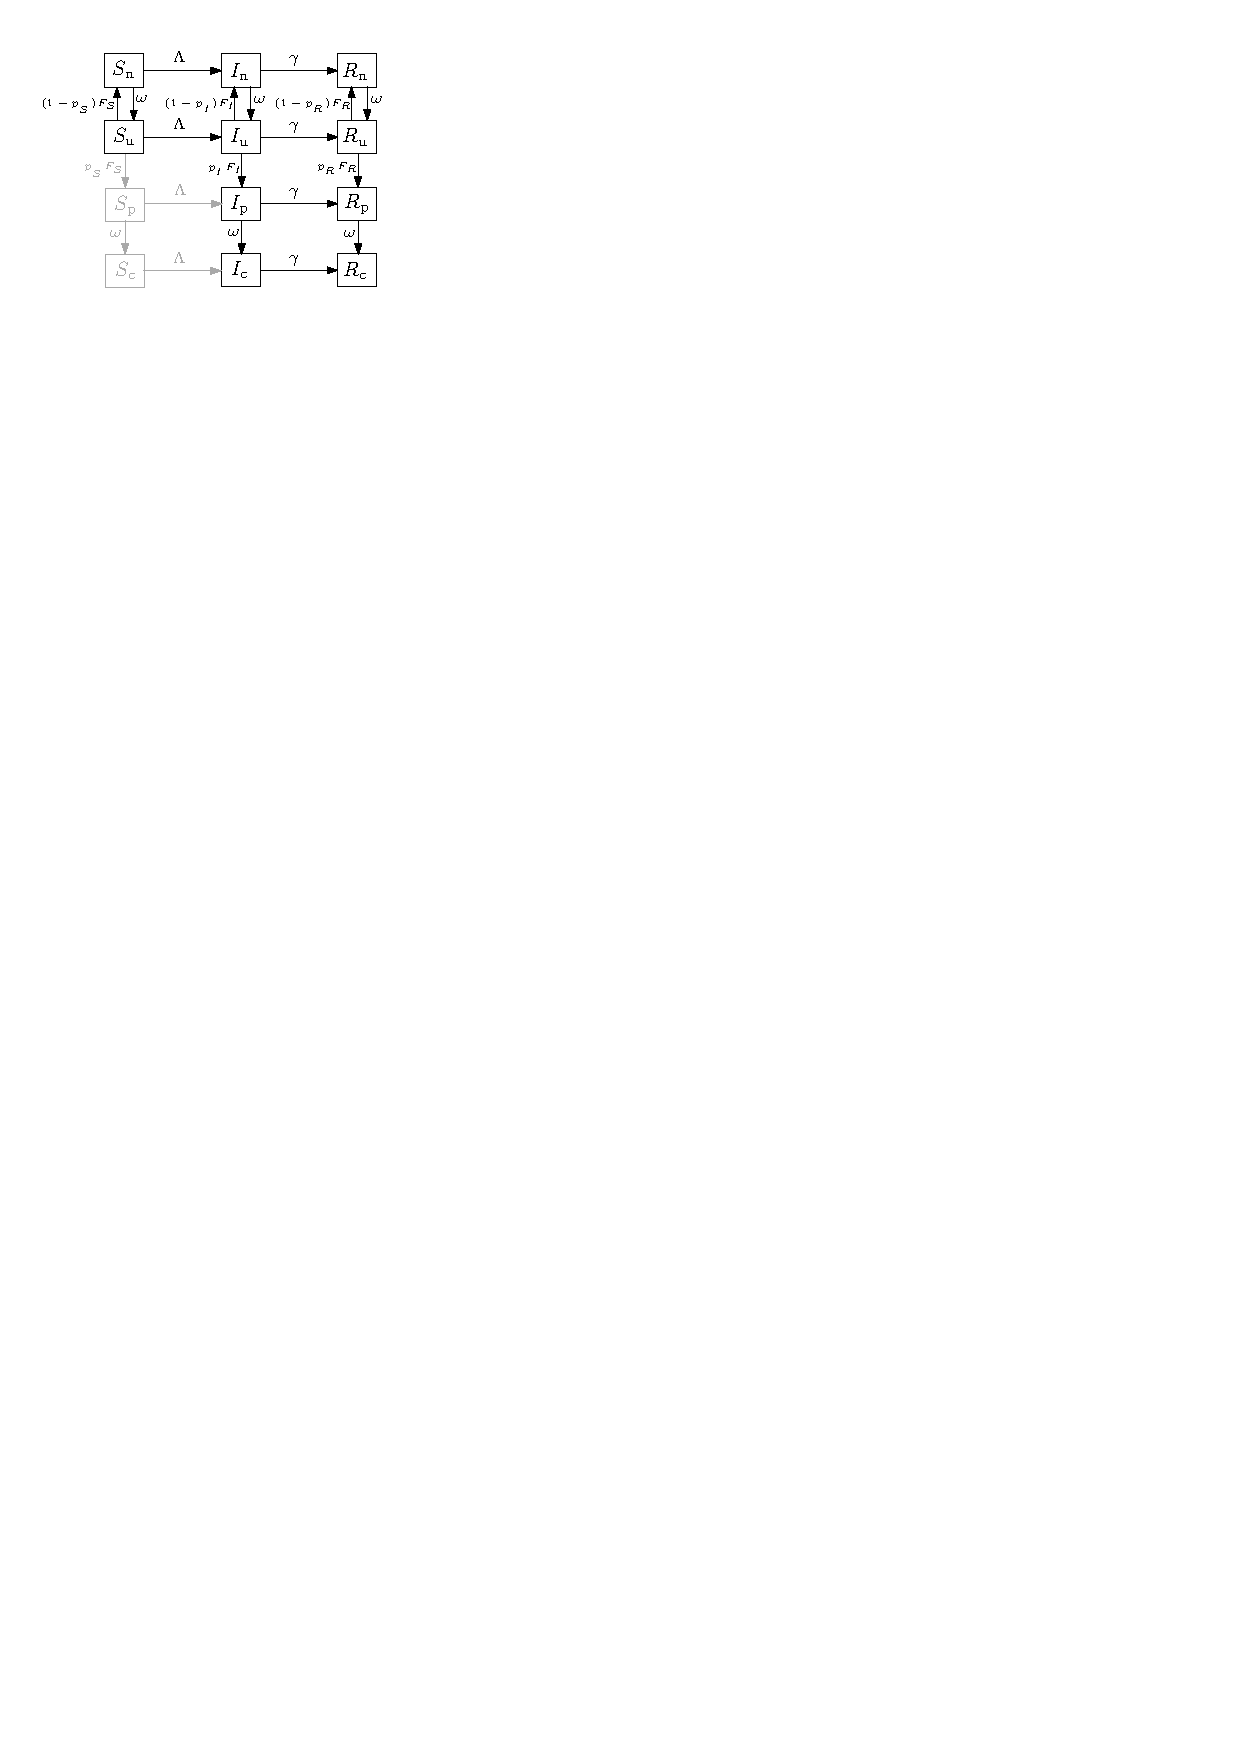
\includegraphics[scale=2]{pix/sir_comp.pdf}
\caption{\small Flowchart of the SIR (Susceptible-Infectious-Recovered) model, \ref{model}. Here, the disease-based status of a compartment $X$, where $X \in \{S,I,R\}$, is combined with the testing-based status including $X\_u$, $X\_p$, $X\_n$ and $X\_c$, for \emph{untested}, waiting-for-\emph{positive}, waiting-for-\emph{negative}, or \emph{confirmed positive}, respectively. Also,  $\Lambda$ is the force of infection with definition in Eq.~\eqref{Lambda}, $\gamma$ is the recovery rate, $\omega$ is the rate of test return, $F_X$ and $p_X$ represent the \percap testing rate and the probability of positive tests, respectively, for compartment $X$. For further description of the parameters see \cref{tab:params}.
\label{fig:flowchart}}
\end{center} 
\end{figure}

Table~\ref{tab:params} defines the model parameters, which are generally straightforward
\percap flows between compartments, or modifiers to these flow rates.  
The novel component of the model comes in through the compartment-specific relative testing weights $w_S$, $w_I$ and $w_R$; these give the relative rates at which people in the $S$, $I$, and $R$ compartments are tested, respectively. For example, $w_I/w_S=2$ means that infected individuals are tested at twice the \percap rate of susceptible individuals. 

In order to link to more applied models, we constructed this model so we could specify the total \percap testing rate. We do this by defining the weighted size of the testing pool $W = w_S S\_u + w_I I\_u + w_R R\_u$, and calculating a scaling parameter for testing as:
\begin{equation}
\label{sigma}
\sigma = \frac{\rho N_0}{W},
\end{equation}
where $\rho$ is the \percap testing rate for population and defined as the number of daily tests taken in a population of size $N_0$.
Thus, the \percap testing rate for compartment $X$ is $F_X=\sigma w_X$, where $X \in \{S,I,R\}$. 
For a high-sensitivity test, infected people typically flow through to the ``confirmed positive'' ($I\_c$, $R\_c$) compartments and are thus unavailable for further testing.  Over the course of the epidemic, a fixed testing rate as specified in \eqref{sigma} can (if large enough) exhaust the pool of people available for testing, leading to a singularity when no one is left untested. Although this phenomenon does not affect our analysis of $\Rnum$, it can affect the temporal dynamics (we discuss an adjustment to the model that solves this problem in the appendix).

The classical SIR model is based on the following implicit assumptions; well-mixed population, homogeneity of the population (i.e., all individuals are equaly susciptable and equaly infectious for the same length of time when infected), exponentially distributed duration of infection and large population size (see, e.g., \cite{keeling2011modeling}). In addition to these standard assumptions, our model, \ref{model}, assumes: (i) there is a single force of infection (new cases per unit time), $\Lambda$, defined as follows
\begin{equation}
\label{Lambda}
\Lambda=\frac{\beta}{N_0} \big(I\_u + (1-\theta\_w)(I\_n+I\_p) + (1-\theta\_c)I\_c \big),
\end{equation}
across all susceptible pools with transmission rate $\beta$ and isolation efficacy in reduction of the probability of transmission for ``waiting'' and \emph{confirmed positive} individuals, $\theta\_w$ and $\theta\_c$ respectively, (see Table~\ref{tab:params} for further details), (ii) $\theta\_c \geq \theta\_w$, i.e., the individuals awaiting test results have a higher transmission probability than the reported individuals. Thus, for instance when the awaiting people follow the isolation perfectly, $\theta\_w$ is closer to 1, while when they less follow the isolation, $\theta\_w$ is closer to 0. For this analysis, we also assume a perfectly specific test ($p_S=0$). This last assumption combined with the assumption that no individual is in waiting-for-\emph{positive} or \emph{confirmed positive} compartments, i.e., $S\_p(0)=S\_c(0)=0$, reduces the model to 10 equations (equations c and d  in \eqref{model} are eliminated).

\begin{table}[htp]
\centering
\begin{tabular}{|c|L{2in}cc|} \hline
  Symbol & Description & Unit & Value \\ \hline
  $N_0$     & Total population size & people & $10^6$ \\ \hline
  $\omega$  & Rate of test return, i.e., rate of onward flow from ``waiting'' to ``confirmed'' or ``untested'' compartments  & 1/day & - \\ \hline
  $\gamma$ & Recovery rate & 1/day & 1/3 \\ \hline 
  $\rho$   & \percap testing rate & 1/day & - \\ \hline 
  $\theta\_w$ & Isolation efficacy in reduction of the probability of transmission for ``waiting'' individuals & - & - \\ \hline
  $\theta\_c$ & Isolation efficacy in reduction of the probability of transmission for ``confirmed positive'' individuals & - & -  \\ \hline
  $\beta$ & Transmission rate & 1/day & 0.39 \\ \hline
  $\Lambda$ & Force of infection & 1/day & - \\ \hline
  $p_S$ & Probability of positive tests for $S$ ($= 1-\textrm{specificity}$) & - & 0 \\ \hline
  $p_I$ & Probability of positive tests for $I$ ($= \textrm{sensitivity}$) & - & 1 \\ \hline
  $p_R$ & Probability of positive tests for $R$ ($= 1-\textrm{specificity}$) & - & 0.5 \\ \hline
  $w_S, w_I, w_R$ & Relative testing weights & - &
  \begin{minipage}[t]{0.21\columnwidth}%
    Random: $\{1,1,1\}$ \\ Targeted: $\{0.3,1,1\}$
  \end{minipage} \\
  \hline
  \end{tabular}
\caption{\label{tab:params} Parameters of the model \eqref{model}.}
\end{table}

The Disease-Free Equilibrium, DFE hearafter, for the SIR model, Eqs. \eqref{model}, is given by setting the differential equations to 0 and solving for the unknowns. The DFE is
\begin{equation}
\label{dfe}
S\_n^*= \frac{\rho}{\omega} N_0, \ S\_u^*= N_0-S\_n^*, \text{~and~} I_j=R_j=0 \ \text{for all }j.
\end{equation}
For brevity, we write 
\begin{equation}
\label{eq:fi}
\hat F_I = (\omega\rho/(\omega-\rho))w_I/w_S
\end{equation}
for the \percap testing rate of infectious individuals near the disease-free equilibrium.

The basic reproduction number, $\Rnum$, was calculated by using the next generation matrix method developed by \cite{van2002reproduction}. $\Rnum$ is
\begin{equation}
\label{R0}
\Rnum= \frac{\beta}{\gamma} (1-\Delta), 
\end{equation}
where the term $\frac{\beta}{\gamma}$ is the classical basic reproduction number for a SIR model without testing and isolation \todo{ref?}, and $\Delta$ is the reduction parameter defined as follows.
\begin{equation}
\label{eq:Delta1}
\Delta= (A~ \theta\_w + B~ \theta\_c) / C,
\end{equation}
where
\begin{equation}
\begin{aligned}
\label{eq:abc}
A=& \gamma \Big( \big(\gamma(\omega+\gamma) + \omega p_I \hat F_I \big) \frac{S\_n^*}{N_0} + (\omega+\gamma) \hat F_I \Big),\\
B=& \omega p_I(\gamma \frac{S\_u^*}{N_0}+\omega)\hat F_I, \\ 
C=& (\omega+\gamma) \Big(\gamma(\omega+\gamma)+(\gamma+\omega p_I)\hat F_I\Big).
\end{aligned}
\end{equation}
Further details of derivation of $\Rnum$ are provided in the appendix section \ref{app:R0}.
 
The analytical calculation of the next-generation matrix and the derivation of $\Rnum$ was carried out in Maple \citep{maple14}. 
We used R \citep{r} for simulations and for plotting $\Rnum$ as a function of the underlying parameters. In particular, the contours of $\Delta$ \eqref{eq:Delta1} were plotted for a combination set of parameters with the baseline parameter values are presented in Table~\ref{tab:params} and isolation efficacy parameters, $\theta\_w$ and $\theta\_c$ vary from 0 to 1.
Results are shown in Figures \ref{pan} and \ref{pan2}, where  panel (a) represents the random testing ($w_S=w_I=w_R=1$), and panel (b) is representing non-random testing ($w_S=0.3$ and $w_I=w_R=1$). 
Fig. \ref{pan} reflects the changes in $\Rnum$  when the \percap testing rate is small relative to the population size, $\rho \in [0,0.01]$, and the test return rate $\omega\in [0.1,2]$.  
Fig. \ref{pan2} reflects the changes in $\Rnum$  when the \percap testing rate is large relative to the population size, $\rho \in [0,0.5]$, and the test return rate $\omega\in (0.5,2]$. 
Note that the critical contour of $\Delta=1-\frac{\gamma}{\beta}$, corresponding to $\Rnum=1$, is plotted in solid line in the Figures. 

% %%%%%%%
\section{Results}

The explicit formula for the basic reproduction number, $\Rnum$ \eqref{R0}, provides an opportunity to study the influence of changes in the underlying parameters on the critical index of epidemic dynamics. We are interested in exploring the effect of parameters that could be manipulated by public-health policy, including the isolation efficacy parameters, $\theta\_c$ and $\theta\_w$, \percap testing intensity, $\rho$, and the test return rate, $\omega$.

Examining our formula for $\Rnum$ \eqref{R0} gives the following results. 
See the appendix for details.

\begin{enumerate}
\item \label{p1:eta} increasing the isolation parameters for tested and confirmed individuals decreases \Rnum;
$$\partial{\Rnum}/\partial{\theta\_c} \leq 0 \text{~and~} \partial{\Rnum}/\partial{\theta\_w} \leq 0.$$ 
\item \label{p1:rho} a higher rate of testing may increase or decrease $\Rnum$;
$$\partial{\Rnum}/\partial{\rho} \text{~can be positive or negative}.$$
\item \label{p1:omega} A higher rate of of test return may increase or decrease \Rnum.
$$\partial{\Rnum}/\partial{\omega} \text{~can be positive or negative}.$$
\end{enumerate}

\begin{figure}[h!]
\centering
\begin{subfigure}[t]{.45\textwidth}
\centering
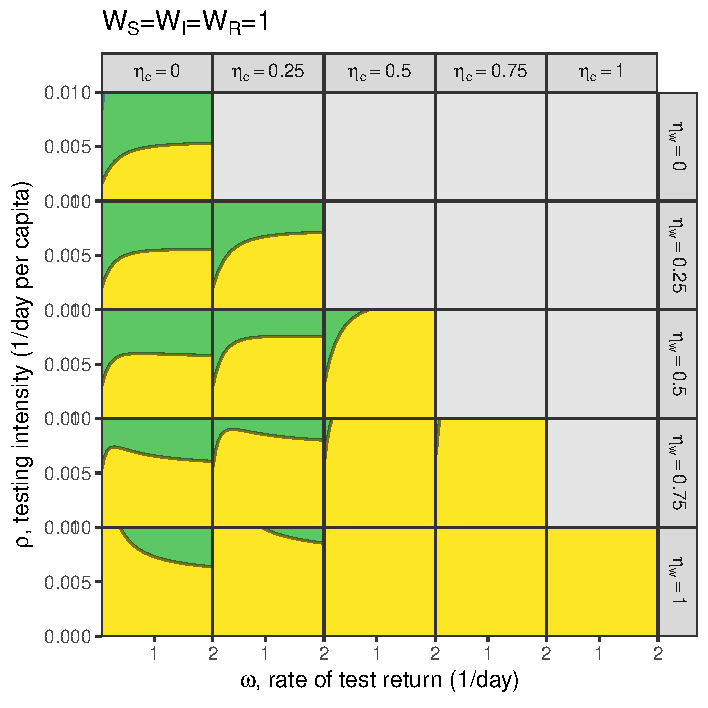
\includegraphics[width=\linewidth]{codes/R0contour_random.pdf}
\caption{}\label{p.a}
\end{subfigure}
%
\begin{subfigure}[t]{.45\textwidth}
\centering
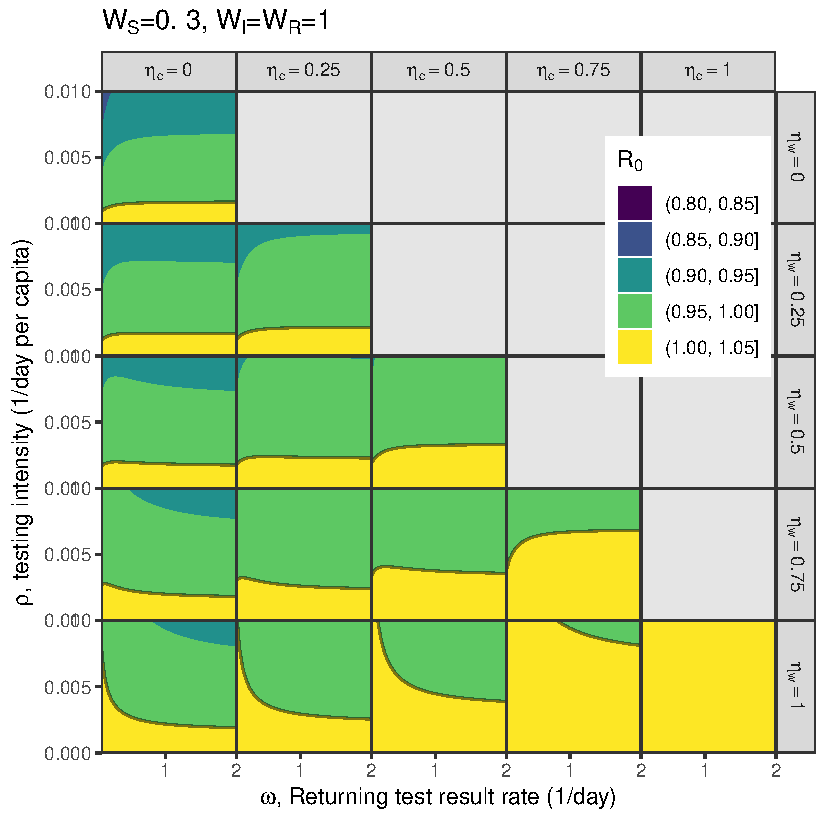
\includegraphics[width=\linewidth]{codes/R0contour_TTI.pdf}
\caption{}\label{p.b}
\end{subfigure}
\caption{
{\bf A comparison of the behaviour of the basic reproduction number, $\Rnum$, between random versus targeted testing strategies at different levels of testing and isolation.}
We numerically evaluate $\Delta$ \eqref{R0}, reflecting the reduction of $\Rnum$ with respect to testing and isolation. We use the following parameters (see Table \ref{tab:params}):
$N_0=1 \times 10^6$, $\omega \in [0.1,2]$ 1/day, $1/\gamma= 3$ days, $\rho \in [0,0.01]$ 1/day, $\theta\_w$ and $\theta\_c$ vary between 0 and 1 with 0 for no effect and 1 for full effect of isolation on the transmission probability, $\beta=0.39$ 1/day, $p_S=0$, $p_I=1$ and $p_R=0.5$. Contours of $\Delta$ are plotted for two testing strategies identified by a set of relative testing weights; (a) random testing where $w_S=w_I=w_R=1$ and (b) targeted testing where $w_S=0.3$ and $w_I=w_R=1$. The black solid line in each panel represents the critical contour of $\Delta=1-\frac{\gamma}{\beta}$, i.e., the $\Delta$ corresponding to the threshold of $\Rnum=1$. \bmb{we still have some collisions in the y-axis tick labels}
}
\label{pan}
\end{figure}

Our numerical results are shown in Figure \ref{pan}. It can be inferred that when random testing strategy is applied, Figure \ref{p.a}, comparing to the targeted testing strategy, Figure \ref{p.b}, the critical \percap testing intensity of the corresponding panels are lower in non-random testing. Also, it appears that speeding the test reporting, i.e., increasing $\omega$, does not significantly lower $\Rnum$ when awaiting people (including people in $I\_p$ and $I\_n$ compartments) follow the isolation perfectly, i.e., $\theta\_w$ is closer to 1. However, speeding the test reporting reduces the epidemic more when the awaiting people less follow the isolation, i.e., $\theta\_w$ is closer to 0. 

Furthermore, we derived an inequality that quantifies the exact relationships between model parameters that result in returning tests more rapidly being favorable \eqref{eq:necsuf}.
\david{What do we learn from this inequality?  Why is it relegated to an appendix?}

%%%%%%%%%%%%
\section{Discussion}

Mathematical modeling of infectious disease outbreaks provides insights on how testing processes influence the epidemiological processes through isolation. 
Here, we develop a compartmental SIR-type model to study the potential effect of testing strategies, testing intensity, test sensitivity and specificity, test reporting time and isolation on epidemic dynamics. 
While targeted testing strategies 
\david{you need to be clearer: you mean targeting individuals who have contacted people who were infected.  For example, here you could say something like ``While targeting the contacts of confirmed cases\dots''}
are always more effective than random testing, as expected, we find that in some cases the direct effect of testing is that viral spread
is greater for a slow test than for a fast test. This counter-intuitive effect can occur when people are cautious when awaiting a test result, and may not be robust to second-order effects of fast testing (such as better contact tracing).

We incorporated the compartment-specific relative testing weights, $w_S$, $w_I$ and $w_R$, to model random testing and \emph{targeted} testing strategies. Here, in the case of targeted testing and for the simplicity and illustration purposes, we assumed that infected and recovered individuals are tested at three times the \percap rate of susceptible individuals, thus $w_I/w_S=3$ and $w_R=w_I$. Note that we have not specified a methodology to assign particular relative testing weights corresponding to a particular targeted testing scenario. 
This part needs to be developed further in future work. 
Modeling different targeted testing strategies, equivalently test-specific testing weights in our framework, requires prior information of the conditional probabilities of getting tested for people in a given compartment. 
This can be implied when we would like to quantify and compare the effect of different levels of test focus for infectious people on the basic reproduction number $\Rnum$, and conclude about the disease spread management. For example, when people are tested for "screening", the individuals with potential higher mobility, eg. people who are getting on flights, get more tested and thus the coresponding heavier testing weight is assigned than people awaiting for a surgery and are probably going to stay in a long-term care facility and consequently less mobile and more isolated to begin with. With our model, we would be able to compare the sensitivity of the disease dynamics, through $\Rnum$, with respect to testing processes.

{\bf The \percap testing intensity, $\rho$;}
Proposition \ref{prop1} part \ref{p1:rho} and also Figure \ref{pan} indicates that increasing testing intensity $\rho$ reduces $\Rnum$. This is sensible since as people are moved to test compartments, namely $X_p$ and $X_n$ for $X \in \{S,I,R\}$, they may partially or fully self-isolate. Also individuals who have tested positive, namely $X_c$ compartment for $X \in \{S,I,R\}$, are highly likely to self-isolate. The higher probability of being subject to isolation, the lower the force of infection \eqref{Lambda} and the lower $\Rnum$ will become. While our simulation supported this result, analytically it appeared to be hard to conclude this due to the complexity of $\Rnum$ expression.  

{\bf The potential advantage of slow test reporting, or favorable-delay-reporting;}
Individuals are highly likely to fully self-isolate when they are either awaiting the test results or they are reported, thus reducing or eliminating their potentially infectious contacts. Thus, the faster the test reporting rate, $\omega$, the shorter these individuals stay in the ``\emph {safe}'' awaiting-confirmed compartments, namely $X_n$, $X_p$ and $X_c$ for $X \in \{S,I,R\}$, and the more they get involved in the infection process.
This advantage of slow test reporting is real, and neglected. 
We also compare to an individual-level advantage of fast tests: people who test positive may be even more careful.
In our model analysis, Proposition \ref{prop1} part \ref{p1:omega} is describing this potential advantage. 
It states that returning test results more rapidly, i.e., increasing the rate $\omega$, does not necessarily lower the reproduction number $\Rnum$; whether increasing $\omega$ lowers $\Rnum$ depends on the precise combination of model parameters  including test reporting rate, testing strategies represented by compartment-specific testing weights, test sensitivity and specificity, and the level of isolation. 
Specifically, in the case of perfect isolation, i.e., when $\theta\_w=1$ and $\theta\_c=1$, $\Rnum$ may increase as the test reporting process becomes faster. This can be seen from expression \eqref{Rom}.
Another example of this favorable delay in $\omega$ could be when the test being employed produces many false negatives. Because many infected asymptomatic individuals will believe they are uninfected/uninfectious, thus may unknowingly spread the virus to many others. Again the delay in the test reporting rate keeps these individuals in the ``\emph {safe}'' awaiting-confirmed compartments.  

we are missing out on
community-level advantages of fast testing: better assessment of the
situation, identification of hot spots, contact-tracing, etc.
The \percap testing intensity of CIVID-19 after about a year from the first case reported in December 2019, is still low (($\rho \approx 0$) in our model). In near future new test kits may be widely accessible, our model provide insights in this case. 
In particular, if a cheap test can identify on average more infected individuals as an expensive test, then our model predicts that the cheap test will lower $\Rnum$ more. In contrast, if an expensive test can identify on average more infected individuals, it will not necessarily lower $\Rnum$ more than the cheap test. The use of tests cheaper than RT-PCR has been proposed as a potential strategy for containing the COVID pandemic. While cheaper tests may be less sensitive and reliable than RT-PCR, they allow for broader and more intense testing. Using our Taylor approximation of $\Rnum$ near $\rho = 0$, we examined what circumstances (i.e., model parameters) make the use of one test more favourable than another, and give a complete description through inequality \ref{eq:rho1vsrho2}. In general, we found that the expensive test tends to more effectively lower $\Rnum$ when (a) individuals who test positive self-isolate much more than individuals who are waiting for their test result, (b) the time it takes to return tests is much shorter than the mean infectious period, and (c) the testing intensity is much greater for infected individuals than susceptible individuals.

\ali{ not sure if we want these 2 following parageraphs, or shrink it into afew short sentences?}
In addition to the favorable-delay-reporting observation of our model \eqref{model}, the model enables us to quantify the amount of delay required in the test reporting process as a strategy to reduce $\Rnum$.
To give a biological interpretation, we describe the qualitative trends predicted by the inequality \eqref{eq:necsuf}. To summarise, returning test results more rapidly tends to be favourable (i.e., reduces $\Rnum$) when (i) \emph{Confirmed-positive} individuals, lower their contact much more than individuals who are waiting for their test results (i.e., $\theta\_c \gg \theta\_w$), (ii) the test is highly sensitive (i.e., $p_I$ is close to 1), and (iii) the targeted testing strategy is used (i.e., $w_I \gg w_S$). 

one point we can make when discussing the relative weight of testing in different compartments is to discuss pre-testing screening tools, such as surveys or questionnaires. If we have a quantitative description of how the testing intensities affect the dynamics, we can make statements like ``our results suggest that employing a pre-testing screening tool can help target infected individuals more effectively. In particular, doubling the sensitivity of the pre-screening tool would *do something* to $\Rnum$.

\david{Some of this reads like notes for discussion rather than text for the paper, so I'm not trying to edit.}

% %%%%%%%
\bibliography{SIRlibrary}

% %%%%%%%%%%%%%%%%%%%%%%%%%%%%%%%%%%%%%%%%%%%%%%%%%%%%%%%%%%%%%%%%%%
\clearpage
% \widetext
\begin{center}
\textbf{\large Appendix}
\end{center}
\setcounter{equation}{0}
\setcounter{figure}{0}
\setcounter{table}{0}
% \setcounter{page}{1}
\makeatletter
\renewcommand{\theequation}{A\arabic{equation}}
\renewcommand{\thefigure}{A\arabic{figure}}
\renewcommand{\bibnumfmt}[1]{[A#1]}
\renewcommand{\citenumfont}[1]{A#1}

\subsection{Model and calculation of $\Rnum$}\label{app:R0}

The model in the form of a system of ordinary differential equations is 
\begin{subequations}\label{model}
\begin{align}
 d S\_u/dt &= -\Lambda S\_u - F_S S\_u + \omega S\_n, \\
 d S\_n/dt &= -\Lambda S\_n + (1-p_S) F_S S\_u - \omega S\_n, \\
 d S\_p/dt &= -\Lambda S\_p + p_S F_S S\_u - \omega S\_p, \\
 d S\_c/dt &= -\Lambda S\_c + \omega S\_p, \\
 d I\_u/dt &= \Lambda S\_u - F_I I\_u + \omega I\_n  - \gamma I\_u, \\
 d I\_n/dt &= \Lambda S\_n + (1-p_I) F_I I\_u - \omega I\_n -\gamma I\_n, \\
 d I\_p/dt &= \Lambda S\_p + p_I F_I I\_u - \omega I\_p -\gamma I\_p, \\
 d I\_c/dt &= \Lambda S\_c + \omega I\_p - \gamma I\_c, \\
 d R\_u/dt &= \gamma I\_u - F_R R\_u + \omega R\_n, \\
 d R\_n/dt &= \gamma I\_n + (1-p_R) F_R R\_u - \omega R\_n, \\
 d R\_p/dt &= \gamma I\_p + p_R F_R R\_u  - \omega R\_p, \\
 d R\_c/dt&= \gamma I\_c + \omega R\_p, \\
 dN/dt &= \omega (S\_n + I\_n + R\_n),  \\
 dP/dt &= \omega(I\_p + R\_p) ,
\end{align}
\end{subequations}

where parameters are specified in Table \ref{tab:params}. The next generation matrix for this model is $G = F V^{-1}$, where matrix $F$ represents the inflow of new infection to the infected compartments and matrix $V$ represents the flow in the infected compartments when the population is totally susceptible. 
Matrices $F$ and $V$ are
\begin{align}
\label{FV}
F =& \beta/N_0 \left[ \begin {array}{cccc} 
S\_u^* & (1-\theta\_w)\,S\_u^* & (1-\theta\_w)\,S\_u^* & (1-\theta\_c)\,S\_u^*\\
S\_n^* & (1-\theta\_w)\,S\_n^* & (1-\theta\_w)\,S\_n^* & (1-\theta\_c)\,S\_n^* \\ 
0&0&0&0\\
0&0&0&0
 \end {array} \right] \\
 =&\beta/N_0 \left[ \begin {array}{c} S\_u^* \\ S\_n^* \\ 0 \\ 0 \end {array} \right]
        \left[ \begin {array}{cccc} 1, \, 1-\theta\_w, \, 1-\theta\_w, \, 1-\theta\_c \end {array} \right], \text{and}\\  V=&
 \left[ \begin {array}{cccc}  
\hat F_I+\gamma&-\omega&0&0\\
-(1-p_I)\hat F_I&\omega+\gamma&0&0\\
-p_I \hat F_I&0&\omega+\gamma&0\\
0&0&-\omega&\gamma
\end {array} \right].
\end{align}
The matrix inverse of $V$ is 
\begin{align}
\label{vinv}
V^{-1} =&
\frac{1}{\gamma C}
\left[ \begin {array}{cccc}
\gamma(\omega+\gamma)^2 & \gamma\omega(\omega+\gamma)&0&0\\ \noalign{\medskip}
\gamma(\omega+\gamma)(1-p_I) \hat F_I & \gamma(\omega+\gamma)(\hat F_I+\gamma)&0&0 \\ \noalign{\medskip}
\gamma(\omega+\gamma) p_I \hat F_I & \gamma\omega p_I \hat F_I & C \gamma/(\omega+\gamma) & 0 \\ \noalign{\medskip}
\omega(\omega+\gamma) p_I \hat F_I & \omega^2 p_I \hat F_I & C \omega/(\omega+\gamma) & C
\end {array} \right],
\end{align}
where $C= \big( \gamma(\omega+\gamma)+(\gamma+\omega p_I)\hat F_I \big) (\omega+\gamma)$ and $\hat F_I$ is the \percap testing rate for the infected people and represented in Eq. \eqref{eq:fi}. Note that all the columns of matrix $V^{-1}$ summ up to $1/\gamma$.

The particular form of $F$ with two rows of zeros at the bottom results in the following blocked form of matrix $G$.
\begin{equation}
\label{mat:G}
G = \left[ \begin {array}{cc}
G_{11}&G_{12}\\
0&0
\end {array} \right],
\end{equation}
where both blocked matricies $G_{11}$ and $G_{12}$ are 2 by 2. Given the upper triangular form of matrix $G$, the basic reproduction number $\Rnum$ (defined as the spectral radius of matrix $G$) is only determined by the blocked matrix $G_{11}$,
\begin{equation}
\label{G11}
G_{11} = \frac{\beta}{\gamma \, C} 
\left[ \begin {array}{c} (\omega-\rho)/\omega \\ \rho/\omega \end {array} \right]
\left[ \begin {array}{cccc} 1, \, 1-\theta\_w, \, 1-\theta\_w, \, 1-\theta\_c \end {array} \right]
\left[ \begin {array}{cc}
\gamma(\omega+\gamma)^2 & \gamma\omega(\omega+\gamma)\\ \noalign{\medskip}
\gamma(\omega+\gamma)(1-p_I)\hat F_I & \gamma(\omega+\gamma)(\hat F_I+\gamma) \\ \noalign{\medskip}
\gamma(\omega+\gamma) p_I \hat F_I & \gamma\omega p_I \hat F_I \\ \noalign{\medskip}
\omega(\omega+\gamma) p_I \hat F_I & \omega^2 p_I \hat F_I
\end {array} \right].
\end{equation}
It is notable that matrix $F$ \eqref{FV} has rank one and consequently $G_{11}$ does so. That is $G_{11}$ has only one non-zero eigenvalue which is $\Rnum$.

The expression of $\Rnum$ has a complicated form with all of the model parameters involved. This expression can be simplifed and represented given the specific form of matrix $G_{11}$ \eqref{G11}. For the purpose of simplicity we present $\Rnum$ in the manuscript in terms of expressions $A$, $B$ and $C$, specified in \eqref{eq:abc}. This is intended to show that $\Rnum$ decreases as the strength of isolation, shown by $\theta\_w$ and $\theta\_c$, increases.

It remains hard to show that the reproduction number $\Rnum$ is decreasing with respect to \percap testing intensity, $\rho$, and the speed of the test return, $\omega$, for the feasible ranges of the parameters, that is
\begin{align}
\label{cond}
& \omega>0, \\
& 0 \leq \rho<\omega,\\ 
& 0 \leq \theta\_w \leq \theta\_c \leq 1, \\
& \frac{w_I}{w_S}\geq 1.
\end{align}
One way to do such an analysis is based on the fact that $\rho$ is \percap rate so for a large population size, $N_0 \gg 1$, $\rho$ is very small or close to 0, comparing to $N_0$. This provides a base to linearly approximate $\Rnum$ when $\rho$ is close to 0, and use this approximation to analyze the behaviour of $\Rnum$ with respect to $\omega$ (see section \ref{taylor}). 
In the next section we provide an equivalent representation of $\Rnum$ to provide a ground to prove that more testing intensity decreases $\Rnum$ for a general rane of parameters.  

% %%%%%%%
\subsection{More testing intensity may decreases $\Rnum$}

This is to provide a mathematical materials to prove that $\pro \Delta$ can be positive or negative, with $\Delta$ defined in Eq. \eqref{eq:abc}, and thus $\pro \Rnum < 0$, where $\Rnum$ is the basic reproduction number, given in Eqs.\,\eqref{R0}. We can rewrite matrix $G_{11}$ in \eqref{G11} in the following form to simplify the calculations.
\begin{equation}
\label{G112}
G_{11} = \frac{\beta}{\gamma \, C} 
\left[ \begin {array}{c}  (\omega-\rho)/\omega \\ \rho/\omega  \end {array} \right]
\left[ \begin {array}{cccc} 
C-C_1, C-C_1-C_2\end {array} \right],
\end{equation}
where $C$ is the same as the one in Eq. \eqref{eq:abc}, i.e.,
$$C=(\omega+\gamma)(\gamma(\omega+\gamma)+(\omega\,p_I+\gamma)\,\hat F_I),$$
and $C_1$ and $C_2$ are 
\begin{align}
\label{eq:C12}
C_1 =& (\omega+\gamma)(\theta\_w \, \gamma+\theta\_c\, \omega\, p_I) \hat F_I,\\
C_2 =& (\omega+\gamma)\gamma^2\,\theta\_w+(\theta\_w-\theta\_c)\gamma\,\omega\,p_I\,\hat F_I,
\end{align}
where $\hat F_I$ is given in Eq. \eqref{eq:fi}.
$\Rnum$ is in the same form as in Eq. \eqref{R0}  
$$\Rnum= \frac{\beta}{\gamma} (1-\Delta).$$

Let define $\phi = \hat F_S = \frac{\rho \omega}{\omega-\rho}$, thus
\begin{equation}
\label{eq:phi}
\rho=\frac{\omega \phi}{\omega+\phi}.
\end{equation}
Reparametrizing testing rate $\rho$ by $\phi$ in the expression of $\Rnum$, in Eq.\,\eqref{R0}, and applying the derivative with respect to $\phi$ results in the following simplified expression for $\partial\Delta/\partial\phi$.

with an equivalent but simplified $\Delta$ in Eq.\,\eqref{eq:abc} as
\begin{equation}
\label{eq:del3}
\Delta= \frac{K_1\,\phi^2+K_2\,\phi}{K_3},
\end{equation}
where
\begin{align}
\label{eq:K}
K_1=& \frac{w_I}{w_S}\Big(((1+p_I)\omega+\gamma)\gamma\theta\_w+\omega^2 p_I\theta\_c \Big), \\
K_2=& (\omega+\gamma)\Big( (\frac{w_I}{w_S}\omega+\gamma)\gamma\theta\_w + \frac{w_I}{w_S} \omega^2 p_I\theta\_c \Big),\\
K_3=& (\omega+\gamma) \Big((\omega p_I+\gamma)\frac{w_I}{w_S}\phi\,+\,(\omega+\gamma)\gamma \Big)(\omega+\phi).
\end{align}
The derivative is
\begin{align}
\label{eq:dd3dr}
\partial\Delta/\partial\phi=& \frac{1}{d_3} (a_3\,\phi^2+b_3\,\phi+c_3),
\end{align}
where
\begin{align}
\label{eq:abcd2}
a_3=& \frac{w_I}{w_S} \Big((\omega\,p_I+\gamma)(\theta\_w-\theta\_c)\frac{w_I}{w_S}\omega\,p_I+(\gamma\theta\_w+\omega\,p_I\theta\_c)(\omega+\gamma) \Big),\\
b_3=& 2\frac{w_I}{w_S}(\omega+\gamma)\Big( ((1+p_I)\omega+\gamma)\gamma\theta\_w+\omega^2 p_I\theta\_c \Big) ,\\
c_3=& (\omega+\gamma)^2 \Big( (\frac{w_I}{w_S}\omega+\gamma)\gamma\theta\_w + \frac{w_I}{w_S} \omega^2 p_I\theta\_c \Big),\\
d_3=& \frac{(\omega+\gamma)}{\omega\gamma} \Big((\omega p_I+\gamma)\frac{w_I}{w_S}\phi\,+\,(\omega+\gamma)\gamma \Big)^2(\omega+\phi)^2. 
\end{align}

Note that $\phi\geq 0$, also $b_3$, $c_3$ and $d_3$ are all positive. However $a_3$ can be positive or negative.
If $a_3\geq 0$, $\partial\Delta/\partial\phi \geq 0$ for all feasible range of parameters, thus $\pro\Delta \leq 0$. 
If $a_3 < 0$, then the quadratic expression in the numerator of \eqref{eq:dd3dr} has a positive root, $\phi^*$, such that for $\phi>\phi^*$, $\partial\Delta/\partial\phi < 0$. An example of this scenario occures when $\theta\_w=0$ and $\theta\_c=1$, which is illustraited in the top-right panel of the Fig.\,\ref{pan2} panel (b). This is when the strength of isolation for awaiting people is the least, but the most for the confirmed cases. In this case 
\begin{equation}
\label{ineq:a3}
a_3 <0\iff\omega+\gamma<(\omega\,p_I+\gamma)\frac{w_I}{w_S}.
\end{equation}
Given that $\frac{w_I}{w_S}\geq 1$, and $0\leq\,p_I\leq\,1$, this inequality is hold when a perfect sensitive test is used, i.e., $p_I=1$, and a targeted tesing strategy is followed, i.e., $\frac{w_I}{w_S}>1$. \ali{i)what is the interpretation of this? 2) (Ben:) calculate the corresponding eigenvector to $\Rnum$, scale it to 1, and plot the population of each infected compartment, what does this tell us? }

Note that $\rho$ and $\omega$ have similar mechanism in delaying people to get into $I\_c$. The non monotonic countereffect of testing rate and test return rate are not obvious. 
that people in the DFE waiting for negative test, $S_n^*$.
More testing may have a counter effect on $\Rnum$, as if we have more testing we have more people in $S_n^*$ which will take them longer to get to $I\_c$.


more $\rho$ then


% %%%%%%%
\subsection{rate of returning tests} \label{taylor}
\ali{needs editig}
The linearization of $\Rnum$ around $\rho=0$ is
\begin{equation}\label{linearization}
\Rnum \approx \beta/\gamma + \frac{\beta \rho}{\omega (\omega+\gamma) \gamma^2 w_S} \Big(\gamma(-\theta\_w)(\gamma w_S+\omega w_I) + (-\theta\_c)p_I w_I \omega^2 \Big). 
\end{equation}
So when $\rho \approx 0$ we have $$\partial{\Rnum}/\partial{\omega} \approx  \frac{-\beta \rho}{\gamma w_S\omega^2 (\gamma+\omega)^2}  (a \omega^2 + b \omega + c),$$
where $a=(-\theta\_w)w_I-(-\theta\_c)p_I w_I$, $b=2(-\theta\_w)\gamma w_S$ and $c=(-\theta\_w)\gamma^2 w_S$. 

Perhaps counter-intuitively, the equation above does not predict that $\Rnum$ is monotone decreasing with respect to $\omega$. In other words; our model does not predict that returning test results more rapidly \textit{always} lower $\Rnum$. In order to gain insight into this intriguing behavior, we examine the zeroes of $\frac{\partial{\Rnum}}{\partial{\omega}}(\omega)$.
Defining the following quantity, $Q$, will help us write the roots of $\partial{\Rnum}/\partial{\omega}$ neatly as follows.
\begin{align}\label{eq:defQ}
    Q =& \frac{w_I}{w_S}\left(1-\frac{n_t-1}{n_w-1}p_I \right).
\end{align}
With that in mind, we can write the roots of $\partial{\Rnum}/\partial{\omega}$ as
\begin{align}
    \omega_1 =& \frac{\gamma}{-\sqrt{1-Q}-1} \\
    \omega_2 =& \frac{\gamma}{\sqrt{1-Q}-1}.
\end{align}

Note that the zeroes are real if and only if $Q < 1$. Note that have $\theta\_c > \theta\_w$, so if $p_I \approx 1$, we will have $Q < 0 < 1$. Thus, if we assume near-perfect test sensitivity, $\omega_1$ and $\omega_2$ will be real. 

Assuming $\omega_1, \omega_2$ are real, it is easy to confirm that $\omega_1 < 0$ by looking at the denominator. To see that $\omega_2 > 0$, recall that $Q < 0$, so $\sqrt{1-Q} > 1$ and so $\sqrt{1-Q} -1 > 0$. Knowing that $\omega_1 < 0$, the only root of interest (i.e., biologically relevant quantity) is $\omega_2$. 

We can prove that $\partial{\Rnum}/\partial{\omega} > 0$ when $\omega \in (0,\omega_2)$ and $\partial{\Rnum}/\partial{\omega} < 0$ when $\omega \in (\omega_2,\infty)$ by computing the limits of $\partial{\Rnum}/\partial{\omega}$ at $0$ and $\infty$ respectively. So it follows that $\Rnum$ has a global maximum with respect to $\omega$ at $\omega = \omega_2$.

Now we want to characterize the parameter regions on which $\partial{\Rnum}/\partial{\omega} < 0$ (i.e., the conditions under which returning test results more rapidly is favorable). By the previous analysis, this is equivalent to solving for $\omega > \omega_2$. So
\begin{align}
    &\omega > \omega_2 \nonumber \\
    &\omega > \frac{\gamma}{\sqrt{1-Q}-1} \nonumber \\
    &\sqrt{1-Q} > \frac{\gamma}{\omega}+1 \\
    &1-Q > (\frac{\gamma}{\omega}+1)^2.
\end{align}
Substituting in $Q$ from \eqref{eq:defQ} we have
\begin{align}
    &1-\frac{w_I}{w_S}\left(1-\frac{n_{t}-1}{n_{\omega}-1}P_{i}\right)> \left(\frac{\gamma}{\omega}+1\right)^2 \\
    &-\frac{w_I}{w_S}\left(1-\frac{n_{t}-1}{n_{\omega}-1}P_{i}\right)> \left(\frac{\gamma}{\omega}+1\right)^2+1 \\    
    &\frac{w_I}{w_S}\left(\frac{1-n_{t}}{1-n_{\omega}}P_{i}-1\right)> \left(\frac{\gamma}{\omega}+1\right)^2+1\label{eq:necsuf}.
\end{align}
Since all steps in deriving \eqref{eq:necsuf} are reversible, \eqref{eq:necsuf} gives a necessary and sufficient condition for $\omega > \omega_2$, which characterizes when returning tests more rapidly would cause a decrease in $\Rnum$.

% %%%%%%%
\subsection{On Testing Rate and Numerical Singularity}

In this work, we didn't do any numerical solutions for the trajectories in our analysis. However, if one tries to do so there would be a singularity issue to deal with. 
Specifically, the numerical singularity issue with the chosen $\sigma$ \eqref{sigma} is that the population in $S$ compartments appeared to blow up when the DFE is achieved. This is once the only untested people are susceptibles, the FOI will become $\Lambda=0$, testing rate $F_s=\rho N_0/S\_u$. Thus, the first equation of the model \eqref{model} will become
$d S\_u/dt = - \rho N_0 + \omega S\_n$. Thus changes in $S\_u$ will be no longer dependent on $S\_u$ with a linear rate of leaving the $S\_u$ compartment.
IN fact the testing rate, $\sigma$, should be formulated such that people from the untested compartments will not be tested if they are not there.
One way to fix this issue, is to consider a maximum testing rate, $\tau$ (1/day). In general, we want to test at a rate of $\rho$ across the whole population. This won't always be possible, so we impose a maximum rate of $\tau$ per testable person and redefine $\sigma = \frac{\tau \rho N_0}{\tau W + \rho N_0}$, with the assumption that $\tau \gg \rho$. This alteration in $\sigma$, does not change any results related to $\Rnum$, thus we only impose it in the simulation of the epidemic dynamic.

% %%%%%%%
\subsection{Expensive vs.\ cheap tests}

The use of tests cheaper than RT-PCR has been proposed as a potential strategy for containing the \covid pandemic. While cheaper tests may be less sensitive and reliable than RT-PCR, they allow for broader and more intense testing. In the analysis below, we compare the $\Rnum$ predicted by our model depending on the testing strategy. 

Consider a test that allows us to test at rate $\rho_1$ and has sensitivity $P_{i,1}$, and another test that allows us to test at $\rho_2$ and has sensitivity $P_{i,2}$. Suppose that $\rho_1 > \rho_2$. Recall that the linearization of $\Rnum$ around $\rho \approx 0$ is given by $$\Rnum \approx \beta/\gamma + \frac{\beta \rho}{\omega (\omega+\gamma) \gamma^2 w_S} \Big(\gamma(-\theta\_w)(\gamma w_S+\omega w_I) + (-\theta\_c)p_I w_I \omega^2 \Big).$$


Treating $\Rnum$ as a function of $\rho$ and $P_i$,we can reduce the inequality $$\Rnum(\rho_2, p_{I,2}) < \Rnum(\rho_1, p_{I,1})$$ into 

\begin{align}\label{eq:rho1vsrho2}
    &\rho_1\left(\gamma(-\theta\_w)(\gamma w_S + \omega w_I) + (-\theta\_c)p_{I,1}w_I\omega^2\right) - \rho_2\left(\gamma(-\theta\_w)(\gamma w_S + \omega w_I) + (-\theta\_c)p_{I, 2}w_I\omega^2\right) > 0 \nonumber \\
    &\vdots \nonumber \\
    &\frac{\rho_2P_{i, 2}-\rho_1P_{i, 1} }{\rho_1-\rho_2} > \frac{\theta\_w}{\theta\_c}\cdot \frac{\gamma(\gamma w_S + \omega w_I)}{\omega^2 w_I}
\end{align}

Note that the RHS is positive, thus a necessary condition for the inequality above to hold is that $\rho_2P_{i,2} > \rho_1P_{i,1}$, equivalently 

\begin{equation}
\frac{P_{i,2}}{P_{i,1}} > \frac{\rho_1}{\rho_2}.
\end{equation}

To state an example of this, if test $A$ is three times as expensive as test $B$ (and hence one can test three times as many people with test $B$), using test $A$ rather than $B$ will be favorable only if test $A$ is at least 3 times more sensitive than test $B$. Note that this is a necessary but not sufficient condition, so even if test $A$ is three times more sensitive, it is still possible for test $B$ to be more effective. 

\cref{eq:rho1vsrho2} tells us precisely when a test corresponding to $\rho_2, P_{i,2}$ will yield a lower $\Rnum$ than a test corresponding to $\rho_1, P_{i,1}$, where $\rho_1 > \rho_2$. Some of the qualitative \textit{trends} that favor test 2 (the higher-sensitivity test) include

\begin{itemize}
    \item individuals who test positive self-isolate much more than individuals who are waiting for their test result.
    \item the time it takes to return tests is much shorter than the mean infectious period.
    \item the testing intensity is much greater for infected individuals than susceptible individuals.
\end{itemize}

\subsection{Simulation with $\rho$ varies from 0 to 0.5 }

\begin{figure}[h!]
\centering
\begin{subfigure}[t]{.45\textwidth}
\centering
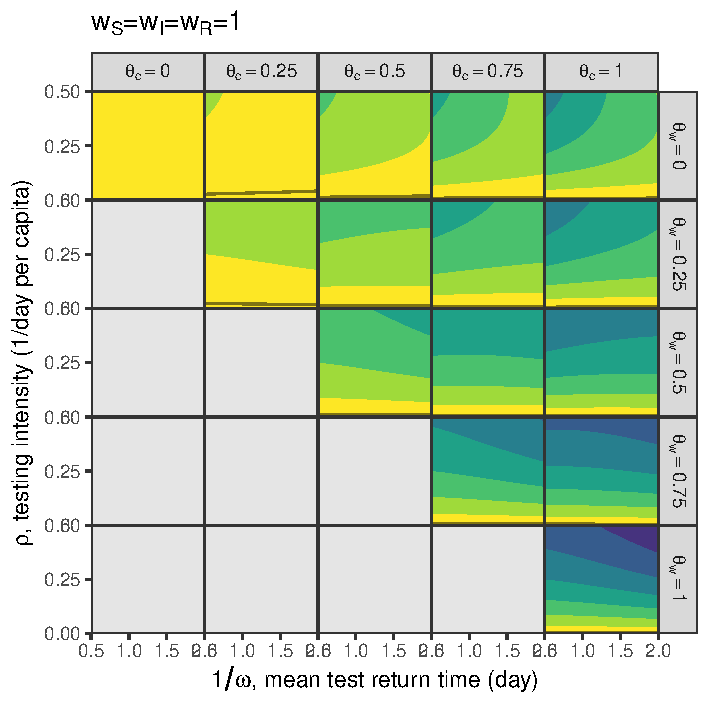
\includegraphics[width=\linewidth]{codes/R0contour_random_rho.5.pdf}
\caption{}
\end{subfigure}
%
\begin{subfigure}[t]{.45\textwidth}
\centering
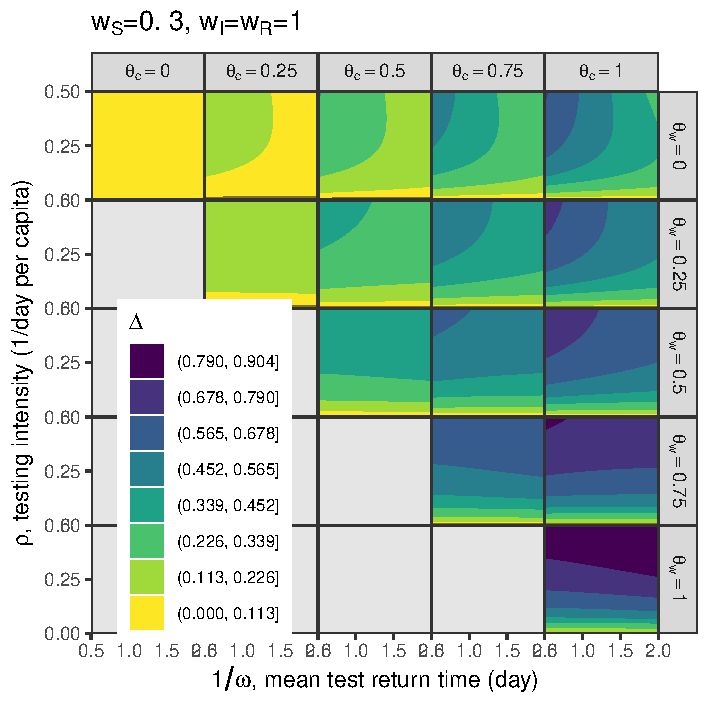
\includegraphics[width=\linewidth]{codes/R0contour_TTI_rho.5.pdf}
\caption{}
\end{subfigure}
\caption{
{\bf A comparison of the behaviour of the basic reproduction number, $\Rnum$, between random versus targeted testing strategies at different levels of testing and isolation.}
We numerically evaluate $\Delta$ \eqref{R0}, reflecting the reduction of $\Rnum$ with respect to testing and isolation. We use the following parameters (listed in Table \ref{tab:params}):
$N_0=1 \times 10^6$, $\omega \in (0.5,2]$ 1/day, $1/\gamma= 3$ days, $\rho \in [0,0.5]$ 1/day, $\theta\_w$ and $\theta\_c$ vary between 0 and 1 with 0 for no effect and 1 for full effect of isolation on the transmission probability, $\beta=0.39$ 1/day, $p_S=0$, $p_I=1$ and $p_R=0.5$. Contours of $\Delta$ are plotted for two testing strategies identified by a set of relative testing weights; (a) random testing where $w_S=w_I=w_R=1$ and (b) targeted testing where $w_S=0.3$ and $w_I=w_R=1$. The black solid line in each panel represents the critical contour of $\Delta=1-\frac{\gamma}{\beta}$, i.e., the $\Delta$ corresponding to the threshold of $\Rnum=1$. \bmb{we still have some collisions in the y-axis tick labels}
}
\label{pan2}
\end{figure}


\end{document}
